\section{Elliptic Curve Cryptography}

\subsection{Elliptic Curves}
In Sections 6 and 7, we have described some discrete logarithm based cryptosystems.
Generic descriptions of these cryptosystems assume a cyclic group $\G$ with some 
basic assumptions, namely that the elements of $\G$ can be represented efficiently,
the group operation in $\G$ can be performed efficiently, but $\DLP$ in $\G$ is 
intractable. We have also worked with discrete logarithm based cryptosystems 
using the multiplicative group $\Z_p^*$. This allowed us to realize a 
practical implementation of the protocols and quantify the security of the 
systems. In particular, the index calculus algorithm (with subexponential
complexity) together with Pollard's $\rho$-algorithm (with square root 
complexity) solves $\DLP$ in $\Z_p^*$ by working with the $256$-bit prime 
order subgroup of $\Z_p^*$, where $p$ is a $3072$-bit prime to ensure 
$128$-bit security of DSA. 

In this section, we introduce elliptic curves over finite fields whose points 
form an additive abelian group, which can be used to instantiate discrete 
logarithm based cryptosystems. In fact, elliptic curve groups offer more 
efficient implementations for key agreement, encryption, and digital signature 
algorithms because the best algorithms to solve $\DLP$ in carefully chosen 
elliptic curve groups have square root complexity, as opposed to the algorithms 
with subexponential complexity that solve $\DLP$ in $\Z_p^*$. 

Let $\K$ be a field. For simplicity, we will assume that $\K$ is not of 
characteristic $2$ or $3$. An elliptic curve $E$ over $\K$ is defined by 
a set of the form 
\[ E/\K = \{(x, y) \in \K \times \K : y^2 = x^3 + ax + b\} \] 
for some $a, b \in \K$ such that the cubic polynomial $x^3 + ax + b$
has no repeated roots in the algebraic closure $\overline{\K}$ of $\K$.
Given an elliptic curve $E/\K$ and a field $\bbL$ as an extension of $\K$
(which might be $\bbL = \K$), the set of points in $E$ with coordinates 
in $\bbL$ is defined as 
\[ E(\bbL) = \{(x, y) \in \bbL \times \bbL : y^2 = x^3 + ax + b\} \cup \{\cal O\}, \] 
where ${\cal O}$ is an extra auxiliary point. This point is sometimes 
denoted as $\infty$ because it actually corresponds to the point at infinity 
$[0, 1, 0]$ when $E$ is considered in the projective space through its equation 
\[ Y^2 Z = X^3 + aXZ + bZ^3 \] 
with $a, b \in \K$. In this course, we choose the notation ${\cal O}$ because 
elliptic curve points form an additive abelian group with ${\cal O}$ 
being the identity element, as we will see later. 

\begin{exmp}
    Recall that $\C$ is the algebraic closure of $\R$. 
    \begin{enumerate}[(1)]
        \item $E/\R = \{(x, y) \in \R \times \R : y^2 = x^3 - x\} \cup \{{\cal O}\}$
        is an elliptic curve over $\R$ since 
        \[ x^3 - x = x(x-1)(x+1) \] 
        has three distinct roots in $\C$. In fact, all three roots are in $\R$. 
        \item $E/\R = \{(x, y) \in \R \times \R : y^2 = x^3 + x\} \cup \{{\cal O}\}$
        is an elliptic curve over $\R$ since
        \[ x^3 + x = x(x-i)(x+i) \] 
        has three distinct roots in $\C$. 
        \item $E/\R = \{(x, y) \in \R \times \R : y^2 = x^3\} \cup \{{\cal O}\}$
        is not an elliptic curve over $\R$ since $x^3$ has the repeated root 
        $0$ in $\C$. 
        \item $E/\R = \{(x, y) \in \R \times \R : y^2 = x^3 - (1/3)x + 
        2/27\} \cup \{{\cal O}\}$ is not an elliptic curve over $\R$ since 
        \[ x^3 - \frac13x + \frac{2}{27} = \left(x - \frac13\right)^{\!2}\left(x + \frac23\right) \] 
        has a repeated root in $\C$.
    \end{enumerate}
\end{exmp}

\begin{remark}
    Let $\K$ be a field whose characteristic is not $2$ or $3$. Let 
    $a, b \in \K$. One can show that if 
    \[ x^3 + ax + b = (x - r_1)(x - r_2)(x - r_3) \] 
    in $\overline{\K}$, then $[(r_1 - r_2)(r_1 - r_3)(r_2 - r_3)]^2 = -(4a^3 + 27b^2)$. 
    In particular, we see that 
    \[ E/\K = \{(x, y) \in \R \times \R : y^2 = x^3 - x\} \cup \{{\cal O}\} \] 
    is an elliptic curve if and only if $4a^3 + 27b^2 \neq 0$. 
\end{remark}

\subsection{Elliptic Curve Groups}
Suppose that $\K$ is a field that is not of characteristic $2$ or $3$. 
Let $\bbL$ be a field extension of $\K$. Let $E/\K$ be the elliptic curve 
defined by the equation $y^2 = x^3 + ax + b$, and let $P$ and $Q$ be 
two points on $E(\bbL)$. 

\begin{defn}
    The {\bf geometric sum} of $P$ and $Q$, denoted by $P + Q$, is defined 
    as follows. 
    \begin{enumerate}[(1)]
        \item If $P = {\cal O}$, then $P + Q = Q$. \textbf{Intuition:} ${\cal O}$ 
        acts like the identity element. 
        \item If $Q = {\cal O}$, then $P + Q = P$. \textbf{Intuition:} ${\cal O}$ 
        acts like the identity element. 
        \item If $P = (x, y)$ and $Q = (x, -y)$, then $P + Q = {\cal O}$.
        \textbf{Intuition:} $Q$ acts like the inverse of $P$. 
        \item If $P = (x_1, y_1)$ and $Q = (x_2, y_2)$ with $x_1 \neq x_2$, then 
        we define $P + Q = (x_3, y_3)$ as follows. Let $\ell$ be the line 
        passing through $P$ and $Q$ given by the equation $y = \alpha x + \beta$. 
        Note that 
        \[ \alpha = \frac{y_2 - y_1}{x_2 - x_1}, \quad \beta = y_1 - \alpha x. \] 
        The line intersects $E$ at exactly three points, two of which are 
        already known by construction; they are $P, Q \in \ell \cap E(\bbL)$. 
        Now, we find the third point $(x'_3, y'_3) \in \ell \cap E(\bbL)$. 
        If a point $(x, \alpha x + \beta)$ is on $E$, then 
        \[ (\alpha x + \beta)^2 = x^3 + ax + b. \] 
        Expanding and rearranging the above equation yields 
        \[ x^3 - \alpha^2 x^2 + (a + 2\alpha\beta)x + (b - \beta^2) = 0. \]
        Notice that $x_1$, $x_2$, and $x'_3$ are all roots of the above 
        cubic. By expanding out $(x - x_1)(x - x_2)(x - x'_3)$ and equating 
        it to the cubic, we can deduce that $x_1 + x_2 + x'_3 = \alpha^2$. 
        Hence, we obtain 
        \[ x'_3 = \alpha^2 - x_1 - x_2 = \left( \frac{y_2 - y_1}{x_2 - x_1} \right)^{\!2} - x_1 - x_2. \] 
        Using the fact that $\alpha = (y'_3 - y_1)/(x'_3 - x_1)$, we can write 
        \[ y'_3 = \left( \frac{y_2 - y_1}{x_2 - x_1} \right)(x'_3 - x_1) + y_1. \] 
        In particular, we see that the third point on $\ell$ is 
        \[ R = (x'_3, y'_3) = \left( \left( \frac{y_2 - y_1}{x_2 - x_1} \right)^{\!2} - x_1 - x_2,\,
        \left( \frac{y_2 - y_1}{x_2 - x_1} \right)(x'_3 - x_1) + y_1 \right). \] 
        Finally, we define $P + Q = (x_3, y_3) = (x'_3, -y'_3)$. 
        \textbf{Intuition:} $P + Q$ is the reflection of the point $R$ 
        about the $x$-axis, where $P$, $Q$, and $R$ are three collinear 
        elliptic curve points. 
        \item If $P = Q = (x_1, y_1)$ with $y_1 \neq 0$, then we define 
        $P + Q = (x_3, y_3)$ as follows. Let $\ell$ be the line tangent 
        to the elliptic curve $E$ at the point $P$, given by the equation 
        $y = \alpha x + \beta$. Note that $y^2 = x^3 + ax + b$, so 
        \[ 2y\frac{\dd y}{\dd x} = 3x^2 + a. \] 
        This implies that 
        \[ \alpha = \frac{3x_1^2 + a}{2y_1}. \] 
        The line $\ell$ intersects $E$ at exactly three points; the point $P$ 
        counts with multiplicity $2$. The third point $(x'_3, y'_3) \in \ell 
        \cap E(\bbL)$ can be found similarly to the previous case. Skipping 
        the details, we can write 
        \[ R = (x'_3, y'_3) = \left( \left( \frac{3x_1^2+a}{2y_1} \right)^{\!2} 
        - 2x_1,\, \left( \frac{3x_1^2+a}{2y_1} \right) (x'_3 - x_1) + y_1 \right). \] 
        Finally, we define $P + Q = (x_3, y_3) = (x'_3, -y'_3)$. \textbf{Intuition:} 
        $P + Q = 2P$ is the reflection of the point $R = (x'_3, y'_3)$ about the 
        $x$-axis, where $R$ lies on the line $\ell$ tangent to $E$ at the point $P$. 
    \end{enumerate}
\end{defn}
The below figure gives a geometric illustration of the operations. 
\begin{center}
    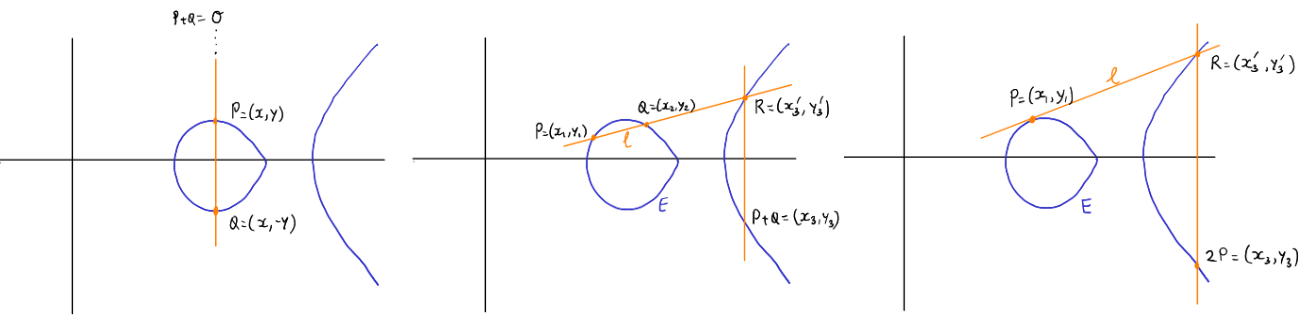
\includegraphics[width=\textwidth]{Images/ec_group_law.png}
\end{center}
One of the most interesting facts about elliptic curves is that the above 
defined geometric sum of points indeed turns the set of points $E(\bbL)$ 
into an abelian group. We explicitly state this in the next theorem, and leave 
the proof as an exercise. 

\begin{thm}
    Define $\K$, $\bbL$, $E/\K$, $E(\bbL)$ and $P + Q$ as above. Furthermore, 
    for $P = (x, y) \in E(\bbL)$, define $-P = (x, -y)$ and $-{\cal O} = {\cal O}$. 
    Then $(E(\bbL), +)$ forms an abelian group. More specifically, 
    given $P, Q, R \in E(\bbL)$, we have the following properties. 
    \begin{enumerate}[(1)]
        \item $E(\bbL)$ is closed under addition: $P + Q \in E(\bbL)$. 
        \item $E(\bbL)$ is associative: $(P + Q) + R = P + (Q + R)$. 
        \item $E(\bbL)$ is commutative: $P + Q = Q + P$.
        \item $E(\bbL)$ has identity element ${\cal O}$: $P + {\cal O} = {\cal O} + P = P$.
        \item Elements in $E(\bbL)$ are invertible: $P + (-P) = (-P) + P = {\cal O}$. 
    \end{enumerate}
\end{thm}

\begin{remark}
    In our above discussion, we have assumed that elliptic curves are 
    defined over fields that are not of characteristic $2$ or $3$. Similar 
    results can still be derived for elliptic curves defined over fields 
    of characteristic $2$ or $3$. In particular, elliptic curve points form 
    a group in these cases as well. However, deriving formulas require a 
    bit more in these cases; see Section 6.7 in \cite{10.5555/1481183}. 
\end{remark}

\subsection{The Size of Elliptic Curve Groups}
Let $\F_p$ be a finite field of size $p$ for some prime $p$. Let $\F_q$ 
be a finite field of size $q$ as a degree $n$ extension of $\F_p$, where 
$q = p^n$ for some positive integer $n$. Recall that finite fields are 
unique up to isomorphism, so we may assume without loss of generality that 
$\F_p = \Z_p$ is the set of integers modulo $p$, and $\F_q = 
\Z_p[z]/\langle f(z) \rangle$ is the polynomial quotient ring of some 
monic irreducible polynomial $f(z)$ of degree $n$ over $\Z_p$. 

For cryptographic purposes, we are mostly interested in elliptic curves 
defined over finite fields. For an elliptic curve $E/\F_p$ defined over 
$\F_p$, the set of $\F_q$-points $E(\F_q)$ forms an abelian group based 
on our results in the previous section, so we can naturally consider 
instantiating discrete logarithm based cryptographic protocols using $E(\F_q)$.
There are many natural questions to ask here. What is the size of 
$E(\F_q)$? What is the group structure of $E(\F_q)$? How difficult is the 
discrete logarithm problem in $E(\F_q)$? 

Let's begin with the size of $E(\F_q)$. Since $E(\F_q)$ contains the 
identity element ${\cal O}$ and the non-identity elements in $E(\F_q)$ 
form a subset of $\F_q \times \F_q$, we can easily obtain the bounds 
\[ 1 \leq |E(\F_q)| \leq q^2 + 1. \] 
Our intuition gives us a better estimate than the one above. If $E/\F_p$ 
is defined by the equation $y^2 = x^3 + ax + b$, then we would expect 
$x^3 + ax + b$ to be a perfect square in $\F_q$ for half of the elements 
$x \in \F_q$. When $x^3 + ax + b$ is a perfect square, then we expect 
exactly two values $y$ to satisfy $y^2 = x^3 + ax + b$, except when 
$x^3 + ax + b = 0$, in which case the unique corresponding value is $y = 0$. 
As a result, we would expect two elliptic curve points for about 
$(q - 1)/2$ choices of $x$, one elliptic curve point for about $1$ choice of $x$,
and no elliptic curve points for about $(q - 1)/2$ choices of $x$. This gives us 
$E(\F_q) \approx q + 1$, counting the identity element ${\cal O}$. It turns 
out that Hasse's theorem confirms this intuition. More precisely, we have 
\[ (\sqrt q - 1)^2 \leq |E(\F_q)| \leq (\sqrt q + 1)^2. \] 
We can use Hasse's theorem to write $|E(\F_q)| = q + 1 + t_q$ for some integer $t_q$ 
such that $|t_q| \leq 2\sqrt{q}$. However, Hasse's theorem only gives us bounds on 
the size of $E(\F_q)$, and it would be convenient to know exactly what that size is. 
Using Schoof's algorithm, we can count the number of points on an elliptic curve in 
polynomial time. Schoof's algorithm and its improvements are beyond the scope of 
the course; we refer to \cite{10.2307/2007968} and 
\href{http://www.mat.uniroma2.it/~schoof/ctpts.pdf}{Schoof's algorithm} for 
the details. Another interesting fact about elliptic curves over finite fields 
is that their group order is somewhat uniformly distributed over Hasse's 
interval $[q + 1 - 2\sqrt{q}, q + 1 + 2\sqrt{q}]$; see Proposition 1.9 in 
\cite{10.2307/1971363}. 

\subsection{Elliptic Curves in Cryptography}
Hasse's bounds on the size of the group of elliptic curves and the somewhat 
uniform distribution of their exact sizes suggests a recipe for choosing a 
suitable elliptic curve to be used in discrete logarithm cryptography. 
\begin{enumerate}
    \item Select a large random prime $p$. 
    \item Select random $a, b \in \F_p$ such that $4a^3 + 27b^2 \neq 0$. 
    \item Let $E_{a,b}/\F_p$ be the elliptic curve defined by the equation 
    $y^2 = x^3 + ax + b$ and count $|E_{a,b}(\F_p)|$. 
    \item If $|E_{a,b}(\F_p)| = h \cdot r$ where $h$ is small (for instance, 
    $1 \leq h \leq 4$) and $r$ is prime, then output $[a, b, p]$; otherwise, 
    go back to step 2. 
\end{enumerate}

\begin{exercise}
    Why do we insist that $h$ is small in $|E_{a,b}(\F_p)| = h \cdot r$? 
\end{exercise}

Once we have chosen $[a, b, p]$ as above, it follows that the elliptic curve 
group $E_{a,b}(\F_p)$ has a cyclic subgroup $\G$ of prime order $r = O(p)$, 
which can be used to initiate discrete logarithm based encryption and digital
signatures (except our group is now additive rather than multiplicative). 
We have seen efficient formulas to perform elliptic group operations, which 
results in efficient elliptic curve discrete logarithm cryptosystems. 

What about the security of such a system? Recall that Pollard's $\rho$-algorithm 
is a general purpose algorithm for solving the discrete logarithm problem, 
so it applies to $\G \subseteq E_{a,b}(\F_p)$ as well, with runtime $O(\sqrt r)$. 
The great thing about the elliptic curve discrete logarithm problem is that 
special purpose subexponential time algorithms, such as the index calculus 
algorithm for solving the discrete logarithm problem in $\F_p^*$, do 
not apply to elliptic curves in general. In other words, the computational 
complexity of the fastest known algorithms to solve the elliptic curve 
discrete logarithm problem in $E_{a,b}(\F_p)$ is $O(\sqrt r) = O(\sqrt p)$. 
Hence, groups obtained from $E_{a,b}/\F_p$ will generally yield comparable 
efficiency and significantly higher security levels than $\F_p^*$. 
More precisely, a carefully chosen elliptic curve over a $256$-bit prime 
provides a security level of $128$-bits. On the other hand, in order to 
achieve the same security level in $\F_p^*$, we require primes $p$ of 
size $3072$-bits. 

\subsection{Pairing-based Cryptography}
Let $\K$ be a field which is not of characteristic $2$ or $3$. Let 
$E/\K$ be an elliptic curve defined by the equation $y^2 = x^3 + ax + b$ 
for $a, b \in \K$. For an integer $n \geq 2$, we define 
\[ E[n] := \{P \in E(\overline{\K}) : nP = {\cal O}\} \] 
to be the set of $n$-torsion points on $E$, where $\overline{\K}$ is the 
algebraic closure of $\K$. It is not hard to check that $E[n]$ is a subgroup of 
$E(\overline{\K})$. Moreover, we can determine $E[2]$ explicitly. 

\begin{exmp}
    Let $\K$ be a field which is not of characteristic $2$ or $3$. Let 
    $E/\K$ be an elliptic curve defined by the equation $y^2 = x^3 + ax + b$ 
    for $a, b \in \K$. As we have seen before, there exist pairwise 
    distinct elements $r_1, r_2, r_3 \in \overline{\K}$ such that 
    $x^3 + ax + b = (x - r_1)(x - r_2)(x - r_3)$. Using the elliptic curve 
    addition laws, we can see that a point $P \in E(\overline{\K})$ 
    satisfies $2P = {\cal O}$ if and only if the tangent line is vertical. 
    This tells us that 
    \[ E[2] = \{{\cal O}, (r_1, 0), (r_2, 0), (r_3, 0)\} \cong \Z_2 \times \Z_2. \] 
\end{exmp}

Similarly, we can show that $E[2] \cong \Z_2 \times \Z_2$ for elliptic curves 
defined over fields of characteristic $3$. The case where the elliptic curve 
is defined over a field of characteristic $2$ is trickier; we can either have 
$E[2] = \{{\cal O}\}$ or $E[2] \cong \Z_2$. In general, we have the following 
result for the $n$-torsion subgroups of elliptic curves. 

\begin{thm}
    Let $E$ be an elliptic curve defined over the field $\K$, and let 
    $n \geq 2$ be an integer. If $\ch(\K) = 0$ or $\ch(\K) \nmid n$, then 
    \[ E[n] \cong \Z_n \times \Z_n. \] 
    Otherwise, we have $\ch(\K) = p \mid n$ and $n = p^rm$ for some $r > 0$ 
    and $m \in \Z$ with $p \nmid m$. In this case, we either have
    $E[n] \cong \Z_m \times \Z_m$ or $E[n] \cong \Z_n \times \Z_m$. 
\end{thm}

Similar to the $n$-torsion subgroup of an elliptic curve, we define the 
$n$-th roots of unity of $\overline{\K}$ to be 
\[ \mu_n = \{g \in \overline{\K} : g^n = 1\}. \] 
Observe that if $\ch(\K) \nmid n$, then the polynomial $x^n - 1$ has no multiple 
roots in $\overline{\K}$ and hence $\mu_n$ forms a cyclic group of order $n$. 
The following theorem shows that $E[n]$ and $\mu_n$ are related through a 
pairing function. 

\begin{thm}[Weil pairing]
    Let $E$ be an elliptic curve defined over the field $\K$, and let 
    $n \geq 2$ be an integer such that $\ch(\K) \nmid n$. Then there exists a 
    Weil pairing function $e_n : E[n] \times E[n] \to \mu_n$ with the following 
    properties:
    \begin{enumerate}[(1)]
        \item $e_n$ is bilinear: for all $P, P_1, P_2, Q, Q_1, Q_2 \in E[n]$, we have 
        \begin{align*}
            e_n(P_1 + P_2, Q) &= e_n(P_1, Q) e_n(P_2, Q), \\ 
            e_n(P, Q_1 + Q_2) &= e_n(P, Q_1) e_n(P, Q_2). 
        \end{align*}
        \item $e_n$ is non-degenerate: if $e_n(P, Q) = 1$ for all $Q \in E[n]$, 
        then $P = {\cal O}$, and if $e_n(P, Q) = 1$ for all $P \in E[n]$, then 
        $Q = {\cal O}$. 
        \item $e_n(P, P) = 1$ for all $P \in E[n]$. 
        \item $e_n(P, Q) = e_n(Q, P)^{-1}$ for all $P, Q \in E[n]$. 
    \end{enumerate}
\end{thm}

Let $E$ be an elliptic curve defined over the field $\K$, and let $n \geq 2$ 
be an integer such that $\ch(\K) \nmid n$. The isomorphism $E[n] 
\cong \Z_n \times \Z_n$ implies that for every $R \in E[n]$, there exists a 
pair of points $P, Q \in E[n]$ and integers $a, b \in \Z$ such that $R = aP + bQ$. In particular, we have 
$E[n] = \langle P, Q \rangle$. It turns out the image of the generators 
$P$ and $Q$ under the Weil pairing function yields a generator for the 
multiplicative group $\mu_n$. 

\begin{thm}
    Let $E$ be an elliptic curve defined over the field $\K$, and let 
    $n \geq 2$ be an integer such that $\ch(\K) \nmid n$. Let 
    $e_n : E[n] \times E[n] \to \mu_n$ be the Weil pairing function. 
    If $E[n] = \langle P, Q \rangle$, then $\mu_n = \langle e_n(P, Q) \rangle$. 
\end{thm}
\begin{pf}
    Let $E[n] = \langle P, Q \rangle$, and suppose that $g = e_n(P, Q)$ 
    has order $d$. Clearly, we have $d \mid n$. For an arbitrary point 
    $R \in E[n]$, we can find $a, b \in \Z$ such that $R = aP + bQ$. 
    We see that 
    \begin{align*}
        e_n(R, dQ) &= e_n(aP + bQ, dQ) \\ 
        &= e_n(aP, dQ) e_n(bQ, dQ) \\ 
        &= e_n(P, dQ)^a e_n(Q, dQ)^b \\ 
        &= e_n(P, Q)^{da} e_n(Q, Q)^{db} \\ 
        &= 1,
    \end{align*}
    where the last equality follows since $g = e_n(P, Q)$ has order $d$ 
    and $e_n(Q, Q) = 1$. Since $R$ is arbitrary and $e_n$ is non-degenerate, 
    we must have $dQ = {\cal O}$. Thus, we must have $n \mid d$ since 
    $Q$ is a point of order $n$. Hence, we obtain $n = d$, as required. 
\end{pf}

Let $E$ be an elliptic curve defined over a finite field $\F_q$, and let 
$n \geq 2$ be an integer such that $\gcd(q, n) = 1$. By Theorem 8.8, we have 
$E[n] \cong \Z_n \times \Z_n$. We further assume that $n \mid |E(\F_q)|$, so 
there exists $P \in E(\F_q)$ such that $P \in E[n]$. Recall that $E[n]$ is a 
subgroup of $E(\overline{\F_q})$. We let $k$ be the smallest positive 
integer such that $E[n] \subseteq E(\F_{q^k})$. In other words, $\F_{q^k}$ 
is the smallest extension of $\F_q$ such that $E(\F_{q^k})[n] \cong \Z_n 
\times \Z_n$. The integer $k$ is called the {\bf embedding degree} of $E$ 
with respect to $n$. One can show that $k$ is also the smallest positive integer 
such that $q^k \equiv 1 \pmod n$. 

Without going into much detail, we note that the Weil pairing function can be 
defined explicitly and that Miller showed how to derive a square-and-multiply 
type algorithm to evaluate pairings in $O(n)$ iterations where a constant 
number of field operations are performed in $E(\F_{q^k})$; see 
\href{https://crypto.stanford.edu/miller/miller.pdf}{Miller's algorithm}.
As a result, the complexity of computing pairings can be written as a polynomial
function of $\log_2(q^k)$. The explicit computation of pairings also allows us to 
see that the output of the pairing function forms a subset of $\F_{q^k}^*$. 
In other words, we can write 
\[ e_n : E[n] \times E[n] \to \mu_n \subseteq \F_{q^k}^*. \] 
Now, we'll discuss two cryptographic applications of pairings. 

\subsubsection{Menezes-Okamoto-Vanstone (MOV) Algorithm}
The first application is due to Menezes, Okamoto, and Vanstone \cite{259647}, 
who showed that one can reduce an instance of an elliptic curve discrete 
logarithm problem (ECDLP) to an instance of a finite field discrete logarithm
problem. More precisely, let $E/\F_q$ be an elliptic curve with a subgroup 
$\G = \langle P \rangle$ of order $n$ generated by $P \in E(\F_q)$, where 
$\gcd(q, n) = 1$. In an instance of ECDLP in $\G = \langle P \rangle$. 
we are given $R \in \G$ and want to recover $a \in \Z_n$ such that $R = aP$. 
We already know how to solve this problem in $O(\sqrt n)$ time by using 
Pollard's $\rho$-algorithm. The MOV algorithm offers an alternative method 
by reducing ECDLP to a discrete logarithm problem in $\F_{q^k}^*$, where 
$k$ is the embedding degree of $E$ with respect to $n$. The steps of 
the MOV algorithm are as follows. 
\begin{enumerate}
    \item Choose a random point $Q \in E(\F_{q^k})[n]$ such that $e_n(P, Q) \neq 1$. 
    \item Compute $g = e_n(P, Q)$ and $h = e_n(R, Q)$. Note that $g, h \in \F_{q^k}^*$. 
    \item Calculate and output the discrete logarithm of $h$ with respect to the base 
    $g$ in $\F_{q^k}^*$. Observe that 
    \[ h = e_n(R, Q) = e_n(aP, Q) = e_n(P, Q)^a = g^a. \] 
\end{enumerate}
The MOV algorithm outperforms Pollard's $\rho$-algorithm for solving ECDLP 
if the underlying elliptic curve has small embedding degree $k$. More precisely, 
this occurs when $k$ is small enough so that the subexponential complexity
of discrete logarithm solvers in $\F_{q^k}^*$ is lower than the exponential 
complexity of Pollard's $\rho$-algorithm, which is $O(\sqrt n)$. In fact, 
there is a class of elliptic curves, called supersingular elliptic curves, 
whose embedding degree is bounded by $k \leq 6$. For supersingular 
elliptic curves, the MOV algorithm yields an ECDLP solver with complexity 
subexponential in $O(\log n)$. 

\subsubsection{Boneh-Lynn-Shacham (BLS) Digital Signature Scheme}
Let $E/\F_q$ be an elliptic curve, and let $n$ be a prime such that 
$n \mid |E(\F_q)|$ and $\gcd(q, n) = 1$. Let $E$ have embedding degree $k$ 
with respect to $n$. We may assume that $E[n] = \langle P, Q \rangle$, where 
$P \in E(\F_q)[n]$, $Q \in E(\F_{q^k}[n]) \setminus E(\F_q)[n]$, and 
$e_n(P, Q) \neq 1$. Under this setting, we can write 
\[ e_n : \langle P \rangle \times \langle Q \rangle \to \mu_n \subseteq \F_{q^k}^*, \] 
which we assume to be publicly available to all the participants of the protocol. 
The Boneh-Lynn-Shacham (BLS) digital signature scheme \cite{10.1007/3-540-45682-1_30}
consists of the following three algorithms. 
\begin{enumerate}
    \item \textbf{Key generation.} The public key and secret key are 
    $\PubKey = R = aQ \in \langle Q \rangle$ and $\SecKey = a \in \Z_n$, where 
    $a$ is chosen uniformly at random. 
    \item \textbf{Signature generation algorithm.} For a given public key 
    $\PubKey = R = aQ$ and the secret key $a$, the signature generation algorithm 
    takes a message $m$ as input, and outputs the signature 
    \[ \sigma = a \cdot H(m) \in \langle P \rangle, \] 
    where $H$ is a cryptographic hash function that encodes messages as elliptic 
    curve points in $\langle P \rangle$.
    \item \textbf{Signature verification algorithm.} For a given public key 
    $\PubKey = R = aQ$, the signature verification algorithm takes the public 
    parameter $Q$, a message $m$, and a signature $\sigma \in \langle P \rangle$ 
    as input. It outputs $\True$ (indicating the validity of the message) if 
    and only if $e_n(\sigma, Q) = e_n(H(m), R)$. Note that for a valid signature, 
    we have 
    \[ e_n(\sigma, Q) = e_n(a \cdot H(m), Q) = e_n(H(m), Q)^a = 
    e_n(H(m), aQ) = e_n(H(m), R). \] 
\end{enumerate}
Notice that a BLS signature consists of a single element $a \cdot H(m)$ as opposed 
to two elements $[r, s]$ as in the ElGamal signature scheme and DSA. As such, 
BLS signatures are also called BLS short signatures. 

For another interesting application of pairings in cryptography, see identity-based 
public key cryptosystems in Section 6.10.2 of \cite{10.5555/1481183}.


